\chapter{Analyse}

 
I dette kapitel vil der kort blive opsummeret, hvad analysearbejdets formål var og de fund denne fase af projektet har affødt. Formålet med analysefasen var  at undersøge og teste om et kendt kredsløb fra artiklen \textit{"Bioimpedance Analysis: A Guide to Simple Design and Implementation"} kan benyttes til at detektere et synk hos raske objekter. Denne artikel er valgt at undersøge, da den indeholder de grundlæggende elementer, der skal være til stede, når der udvikles en BI-sensor. Yderligere har artiklen haft gode erfaringer med at bygge en BI-sensor kredsløb, der er prisbilligt. Se kredsløbet på figur \ref{fig:BIdiagram}. Dette har naturligvis fået projektgruppens opmærksomhed, da projektet kun er budgetteret til kr. 500. Forskerne bag artiklen har udviklet bioimpedans kredsløbet til at måle bioimpedans signaler fra hjernevæv. Om det samme kredsløb kan anvendes til detektering af et synk på en anden vævstype, i dette projektes tilfælde larynx-området, skal denne analysefase undersøge. \\

\begin{figure}[H]
\centering
{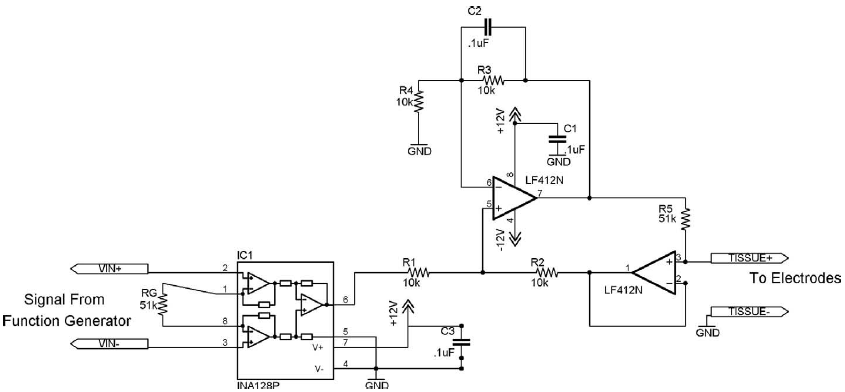
\includegraphics[width=\linewidth]
{Figure/BIdiagram}}
\caption{Diagram over det angivet kredsløb fra artiklen\cite{Aroom2009}}
\label{fig:BIdiagram}
\end{figure}

For at realisere BI-sensoren er der indkøbt præcist de samme elektriske komponenter som artiklens kredsløb gør brug af med undtagelse af udstyr som oscilloskop og funktionsgenerator. Disse udstyr har projektgruppens medlemmer selv anskaffet, se den samlede pris for disse komponenter i \nameref{bilag13}.

For at afgøre, om kredsløbet kan bruges til at detektere et synk, har gruppen bygget kredsløbet på et fumlebræt, og efterfølgende testet det på en af gruppens medlemmer som måleobjekt. Figur \ref{fig:testopstilling1} og \ref{fig:celler} viser, hvordan testopstillingen og implementeringen af BI-kredsløbet ser ud:

\begin{figure}[H]
\centering
{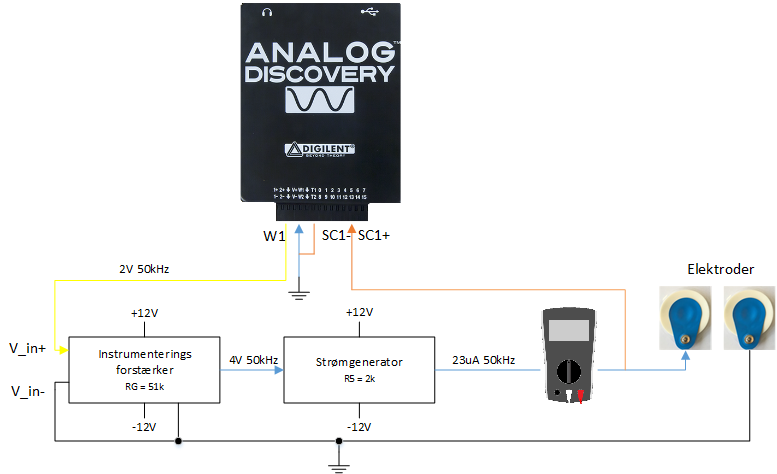
\includegraphics[width=10cm]
{Figure/testopstilling11}}
\caption{Diagram over testopstilling af det angivet kredsløb}
\label{fig:testopstilling1}
\end{figure} 



\begin{figure}[H]
\centering
{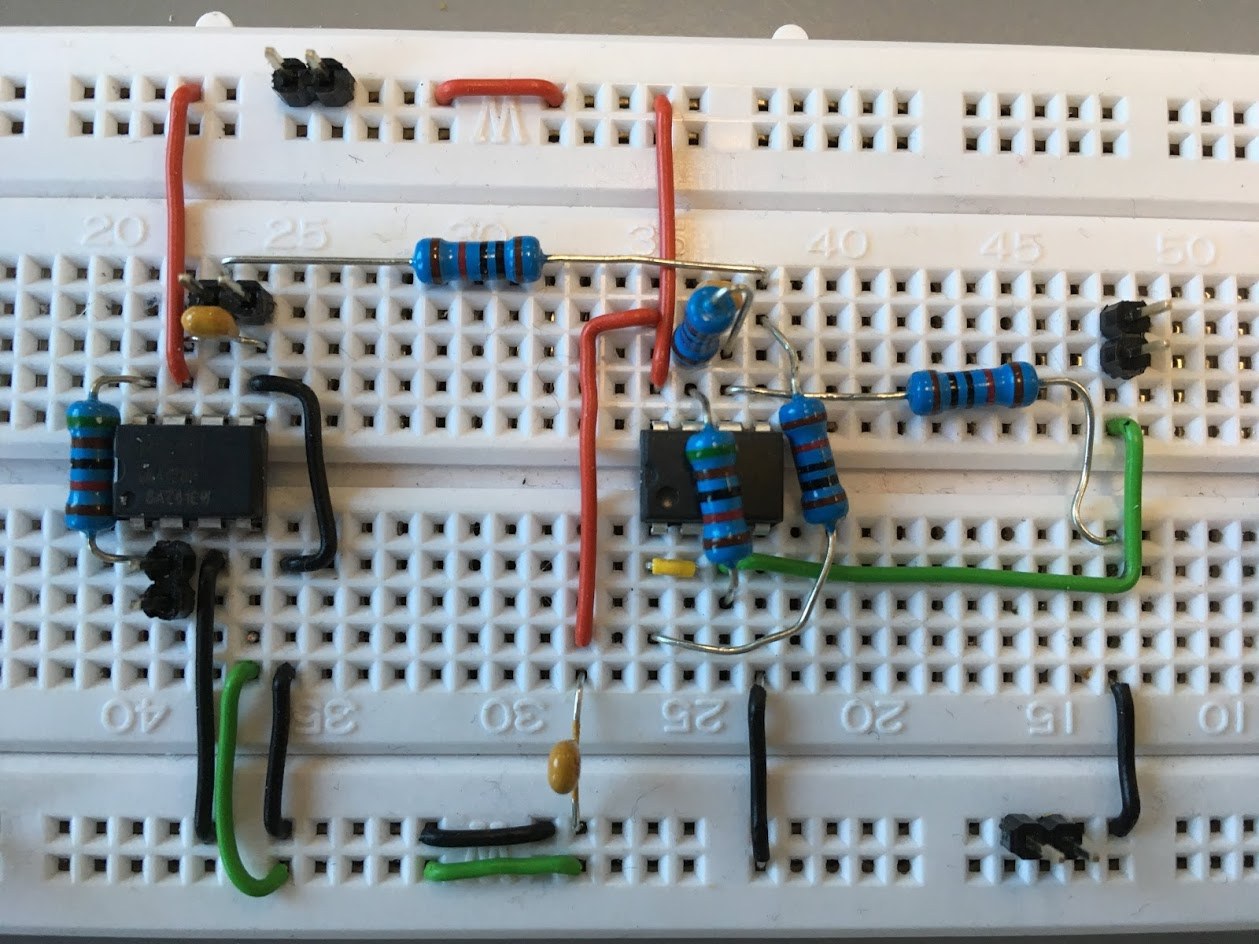
\includegraphics[width=10cm]
{Figure/oprindeligekredslob2}}
\caption{Illustration af testopstillingen på et fumlebræt. Testopstillingen indeholder en instrumentationsforstærker, INA128, til venstre og en strømgenerator, LF412CN, til højre.}
\label{fig:celler}
\end{figure}

Efter testen af kredsløbet, kunne det konstateres at kredsløbet ikke er i stand til at detektere et synk. Se testresultaterne fra BI-kredsløbet på figur \ref{fig:BIdiagram} kan læses i   \nameref{bilag3}.\\

\pagebreak
At systemet ikke er i stand til at detektere et synk kan det bl.a. forklares med følgende:


 
\begin{itemize}
\item at kredsløbet er designede til et andet formål end at detektere et synk
\item at de målte spændinger er så svage at forstærkning af dem er nødvendige
\item at anvendelsen af kun to elektroder påvirker målingernes resultater
\item at artiklen ikke tager højde for undertrykkelse af aliasering
\end{itemize}

Som konsekvens af det manglende synk, besluttede projektgruppen at designe et alternativt BI-kredsløb, der skal detektere et synk. Det nye system skal indeholde følgende komponenter:

\begin{itemize}
\item En funktionsgenerator til at forsyne BI-kredsløbet
\item To instrumentationsforstærkere, der bruges til at forstærke signalet fra funktionsgeneratoren og biosignal fra måleobjektet. De to  instrumentationsforstærkere anvendes desuden til at fjerne 50 Hz brum. 
\item En strømgenerator 
\item 4 Ag/AgCl elektroder til transmittering af strøm og måling af spændinger.
\item En operationsforstærker til at forstærke signalet yderligere for at udnytte ADC'ens spændingsområde mest muligt.

\item Et anti-aliaseringsfilter til at undertrykke aliasering. 
\item En dataopsamlingsenhed

\end{itemize}


 

Med prisen og forhåndskendskabet til nogle af de omtalte komponenter for øje er der valgt at opbygge overstående system  med komponenter, som enten findes på skolens elektronik værksted eller som kan købes billigt. Design og relation mellem overstående komponenter henvises der til \nameref{bilag4} og \nameref{bilag5}. 